
\documentclass[11pt]{article}
% ------- TikZ Preamble -------
\RequirePackage{tikz}
\usetikzlibrary{knots,hobby,calc,intersections,decorations.pathreplacing,decorations.markings,shapes.geometric,spath3}
\tikzset{ knot diagram/every strand/.append style={ultra thick, black}}

\newcommand{\SSTGuidesPoints}[2]{% #1=basename (e.g. P), #2=last index
  \ifsstguides
    \foreach \i in {1,...,#2}{
      \fill[blue] (#1\i) circle (1.2pt);
      \node[blue,font=\scriptsize,above] at (#1\i) {\i};
    }
    \draw[gray!40, dashed]
    \foreach \i [remember=\i as \lasti (initially 1)] in {2,...,#2,1} { (#1\lasti)--(#1\i) };
  \fi
}
% ------- TikZ Preamble -------




% Document
\begin{document}

    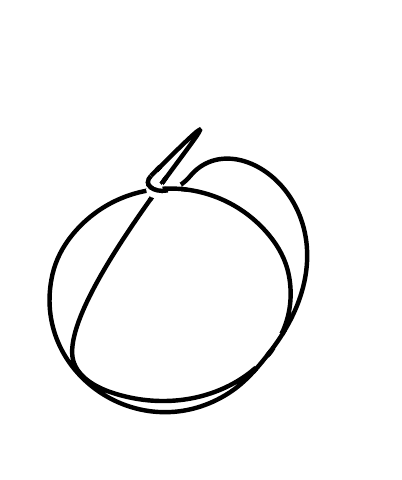
\begin{tikzpicture}[use Hobby shortcut]
    \coordinate (P1) at (-0.25, 1.75);
    \coordinate (P2) at (-1.25, -0.50);
    \coordinate (P3) at (-0.75, -1);
    \coordinate (P4) at (1.50, 0.50);
    \coordinate (P5) at (1.25, 1);
    \coordinate (P6) at (-1.25, 1);
    \coordinate (P7) at (-1.50, 0.50);
    \coordinate (P8) at (0.75, -1);
    \coordinate (P9) at (1.25, -0.50);
    \coordinate (P10) at (0.25, 1.75);
    \coordinate (P11) at (-0.25, 1.75);
    \coordinate (P12) at (-0.25, 1.75); % = P1

    \begin{knot}[
        consider self intersections,
        clip width=5pt, clip radius=3pt,
        ignore endpoint intersections=false,
        flip crossing/.list={2,4,6,8,10,12,14},
        % ----draft mode=crossings % uncomment to see numbers
    ]
    \strand
    ([closed] P1)..(P2)..(P3)..(P4)..(P5)..(P6)..(P7)..(P8)..(P9)..(P10)..(P11)..(P12);
    \end{knot}
% ---- \SSTGuidesPoints{P}{12}
    \end{tikzpicture}



\end{document}